\documentclass[tikz,border=10pt]{standalone}
\usepackage{tikz}
\usetikzlibrary{positioning, arrows.meta, calc, patterns, decorations.pathreplacing}
\usepackage{amsmath}

\begin{document}
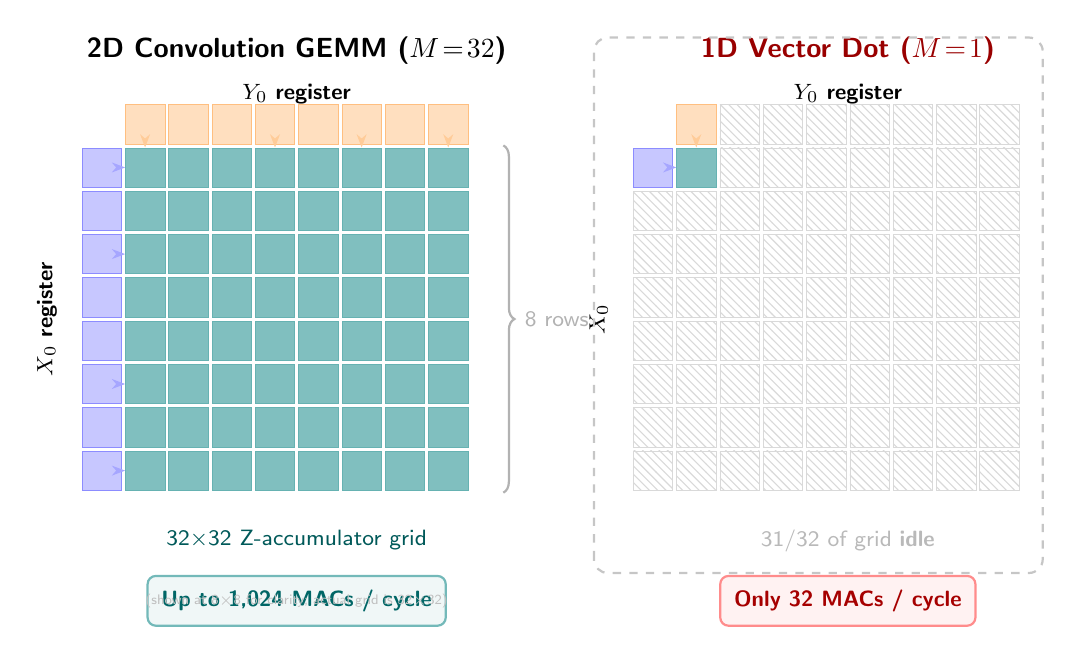
\begin{tikzpicture}[
    >=Stealth,
    font=\sffamily\small,
    cell active/.style={fill=teal!50, draw=teal!60, very thin,
                        minimum size=5mm, inner sep=0pt},
    cell idle/.style={fill=gray!12, draw=gray!30, very thin,
                      minimum size=5mm, inner sep=0pt,
                      pattern=north west lines, pattern color=gray!30},
    reg x/.style={fill=blue!22, draw=blue!45, very thin,
                  minimum size=5mm, inner sep=0pt},
    reg y/.style={fill=orange!25, draw=orange!50, very thin,
                  minimum size=5mm, inner sep=0pt},
]

\def\sz{0.55}  % cell pitch

% =====================================================================
%  LEFT PANEL — Full 8×8 grid (representing 32×32)
% =====================================================================
\begin{scope}[shift={(0,0)}]

    % --- Y register row (top, 8 cells) ---
    \foreach \c in {0,...,7} {
        \node[reg y] (Ly\c) at ({\c*\sz}, {8*\sz}) {};
    }
    \node[above=4pt, font=\sffamily\footnotesize\bfseries] at ({3.5*\sz}, {8*\sz})
        {$Y_0$ register};

    % --- X register column (left, 8 cells) ---
    \foreach \r in {0,...,7} {
        \node[reg x] (Lx\r) at ({-\sz}, {(7-\r)*\sz}) {};
    }
    \node[rotate=90, anchor=south, font=\sffamily\footnotesize\bfseries]
        at ({-\sz - 0.45}, {3.5*\sz}) {$X_0$ register};

    % --- Z accumulator 8×8 grid ---
    \foreach \r in {0,...,7} {
        \foreach \c in {0,...,7} {
            \node[cell active] (Lz\r\c) at ({\c*\sz}, {(7-\r)*\sz}) {};
        }
    }

    % --- Fan arrows: X → grid (a few representative) ---
    \foreach \r in {0,2,5,7} {
        \draw[blue!35, thin, ->] (Lx\r.east) -- (Lz\r 0.west);
    }
    % --- Fan arrows: Y → grid (a few representative) ---
    \foreach \c in {0,3,5,7} {
        \draw[orange!40, thin, ->] (Ly\c.south) -- (Lz0\c.north);
    }

    % --- Brace: "8 rows" ---
    \draw[decorate, decoration={brace, amplitude=4pt, mirror}, thick, gray!60]
        ({8*\sz + 0.15}, 0 - 0.28)
        -- node[right=4pt, font=\sffamily\footnotesize, text=gray!60] {8 rows}
        ({8*\sz + 0.15}, {7*\sz + 0.28});

    % --- Labels below ---
    \node[below=10pt, font=\sffamily\footnotesize, text=teal!70!black]
        at ({3.5*\sz}, -0.28)
        {32$\times$32 Z-accumulator grid};

    \node[below=22pt, draw=teal!55, fill=teal!6, thick, rounded corners=3pt,
          font=\sffamily\footnotesize\bfseries, inner sep=5pt, text=teal!80!black]
        at ({3.5*\sz}, -0.55)
        {Up to 1,024 MACs / cycle};

    \node[font=\sffamily\tiny, text=gray!50] at ({3.5*\sz}, -1.65)
        {(shown at 8$\times$8 for clarity; actual grid is 32$\times$32)};

    % --- Title ---
    \node[above=18pt, font=\sffamily\bfseries] at ({3.5*\sz}, {8*\sz})
        {2D Convolution GEMM ($M\!=\!32$)};
\end{scope}

% =====================================================================
%  RIGHT PANEL — M=1 inset (same 8×8 grid, 1 cell active)
% =====================================================================
\begin{scope}[shift={(7.0, 0)}]

    % --- Y register row (top, 8 cells: 1 active, 7 idle) ---
    \node[reg y] (Ry0) at (0, {8*\sz}) {};
    \foreach \c in {1,...,7} {
        \node[cell idle] at ({\c*\sz}, {8*\sz}) {};
    }
    \node[above=4pt, font=\sffamily\footnotesize\bfseries] at ({3.5*\sz}, {8*\sz})
        {$Y_0$ register};

    % --- X register column (left, 8 cells: 1 active, 7 idle) ---
    \node[reg x] (Rx0) at ({-\sz}, {7*\sz}) {};
    \foreach \r in {1,...,7} {
        \node[cell idle] at ({-\sz}, {(7-\r)*\sz}) {};
    }
    \node[rotate=90, anchor=south, font=\sffamily\footnotesize\bfseries]
        at ({-\sz - 0.45}, {3.5*\sz}) {$X_0$};

    % --- Z grid: (0,0) active, everything else idle ---
    \node[cell active] (Rz00) at (0, {7*\sz}) {};
    % Row 0, cols 1–7: idle
    \foreach \c in {1,...,7} {
        \node[cell idle] at ({\c*\sz}, {7*\sz}) {};
    }
    % Rows 1–7, all cols: idle
    \foreach \r in {1,...,7} {
        \foreach \c in {0,...,7} {
            \node[cell idle] at ({\c*\sz}, {(7-\r)*\sz}) {};
        }
    }

    % --- Arrows ---
    \draw[blue!35, thin, ->] (Rx0.east) -- (Rz00.west);
    \draw[orange!40, thin, ->] (Ry0.south) -- (Rz00.north);

    % --- Labels below ---
    \node[below=10pt, font=\sffamily\footnotesize, text=gray!55]
        at ({3.5*\sz}, -0.28)
        {31/32 of grid \textbf{idle}};

    \node[below=22pt, draw=red!45, fill=red!5, thick, rounded corners=3pt,
          font=\sffamily\footnotesize\bfseries, inner sep=5pt, text=red!65!black]
        at ({3.5*\sz}, -0.55)
        {Only 32 MACs / cycle};

    % --- Title ---
    \node[above=18pt, font=\sffamily\bfseries, text=red!60!black]
        at ({3.5*\sz}, {8*\sz})
        {1D Vector Dot ($M\!=\!1$)};

    % --- Dashed border ---
    \draw[gray!45, thick, rounded corners=5pt, dashed]
        ({-\sz - 0.75}, -1.3) rectangle ({8*\sz}, {8*\sz + 1.1});
\end{scope}

\end{tikzpicture}
\end{document}
